\documentclass{article}

\usepackage{tikz}

\begin{document}
\begin{figure}
\begin{tikzpicture}[node distance=2in]
%\node(a) at (0,0) {a};
%\node(b) at (1,0) {b};
%\node(Fa) at (0,-1){F a};
%\node(Fb) at (1,-1){F b};
\node(xs0) {raw data};
\node(xs1) [below of=xs0] {processed data};
\node(m0) [right of=xs0] {raw model};
\node(m1) [right of=xs1] {processed model};

\draw[->] (xs0) to (xs1);
\draw[->] (xs0) to (m0);
\draw[->] (xs1) to (m1);
\draw[->] (m0) to (m1);
\end{tikzpicture}
\end{figure}


\begin{figure}
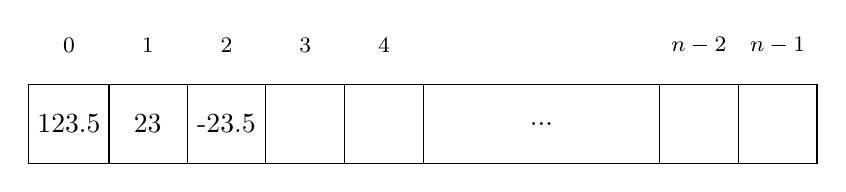
\begin{tikzpicture}
%\node[minimum size=1cm,draw] at (-1.5,0) {6};
%\node[minimum size=1cm,draw] at (-3,0) {8};
%\node at (-1.5,1) {\rotatebox{45}{size}};
%\node at (-2.7,1.2) {\rotatebox{45}{capacity}};

\node[minimum size=1cm,draw] at (0,0) {123.5};
\node[minimum size=1cm,draw] at (1,0) {23};
\node[minimum size=1cm,draw] at (2,0) {-23.5};
\node[minimum size=1cm,draw] at (3,0) {};
\node[minimum size=1cm,draw] at (4,0) {};
\node[minimum size=1cm,minimum width=3cm,draw] at (6,0) {...};
\node[minimum size=1cm,draw] at (8,0) {};
\node[minimum size=1cm,draw] at (9,0) {};

\node at (0,1) {\footnotesize 0};
\node at (1,1) {\footnotesize 1};
\node at (2,1) {\footnotesize 2};
\node at (3,1) {\footnotesize 3};
\node at (4,1) {\footnotesize 4};
\node at (8,1) {\footnotesize $n-2$};
\node at (9,1) {\footnotesize $n-1$};
\end{tikzpicture}
\end{figure}

\begin{figure}
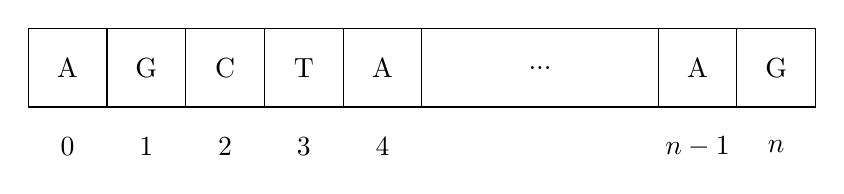
\begin{tikzpicture}
\node[minimum size=1cm,draw] at (0,0) {A};
\node[minimum size=1cm,draw] at (1,0) {G};
\node[minimum size=1cm,draw] at (2,0) {C};
\node[minimum size=1cm,draw] at (3,0) {T};
\node[minimum size=1cm,draw] at (4,0) {A};
\node[minimum size=1cm,minimum width=3cm,draw] at (6,0) {...};
\node[minimum size=1cm,draw] at (8,0) {A};
\node[minimum size=1cm,draw] at (9,0) {G};

\node at (0,-1) {0};
\node at (1,-1) {1};
\node at (2,-1) {2};
\node at (3,-1) {3};
\node at (4,-1) {4};
\node at (8,-1) {$n-1$};
\node at (9,-1) {$n$};
\end{tikzpicture}
\end{figure}

\begin{figure}
\begin{tikzpicture}
\node[minimum height=1cm,minimum width=4cm,draw] at (0,4) {256};
\node[minimum height=1cm,minimum width=4cm,draw] at (0,2) {180};
\node at (-3,4) {capacity};
\node at (-3,2) {size};

\node[minimum height=1cm,minimum width=4cm,draw] at (0,0) {};
\node[minimum height=1cm,minimum width=4cm,draw] at (0,-1) {};
\node[minimum height=1cm,minimum width=4cm,draw] at (0,-2) {};
\node[minimum height=1cm,minimum width=4cm,draw] at (0,-3) {};
\node[minimum height=1cm,minimum width=4cm,draw] at (0,-4) {};
\node[minimum height=3cm,minimum width=4cm,draw] at (0,-6) {...};
\node[minimum height=1cm,minimum width=4cm,draw] at (0,-8) {};
\node[minimum height=1cm,minimum width=4cm,draw] at (0,-9) {};
\node[minimum height=1cm,minimum width=4cm,draw] at (0,-10) {};
\node[minimum height=1cm,minimum width=4cm,draw] at (0,-11) {};
\node[minimum height=3cm,minimum width=4cm,draw] at (0,-13) {...};
\node[minimum height=1cm,minimum width=4cm,draw] at (0,-15) {};
\node[minimum height=1cm,minimum width=4cm,draw] at (0,-16) {};

\node at (-2.5,0) {0};
\node at (-2.5,-1) {1};
\node at (-2.5,-2) {2};
\node at (-2.5,-3) {3};
\node at (-2.5,-4) {4};
\node at (-2.5,-8) {$n-2$};
\node at (-2.5,-9) {$n-1$};
\end{tikzpicture}
\end{figure}

\end{document}
